\section{Results}
\label{sec:results}

In this section, we demonstrate the use of LOBE to block-encode physically-relevant Hamiltonians including an extension of the pairing Hamiltonian used in \cite{liu2024efficient} which includes bosons as well as the $\phi^4$ model used in \ws{insert-blah here @gus @kamil}.
We study both variants of the block-encoding described in Sections \ref{sec:block-encoding} and expanded upon in Section \ref{sec:lobe} and give numerical counts for the numbers of non-Clifford operations, the number of ancillae required beyond the system register, and the rescaling factor imposed on the resulting block-encoding.

\subsection{Pair Production/Annihilation}

\begin{figure}[h]
    \label{fig:feynman}
    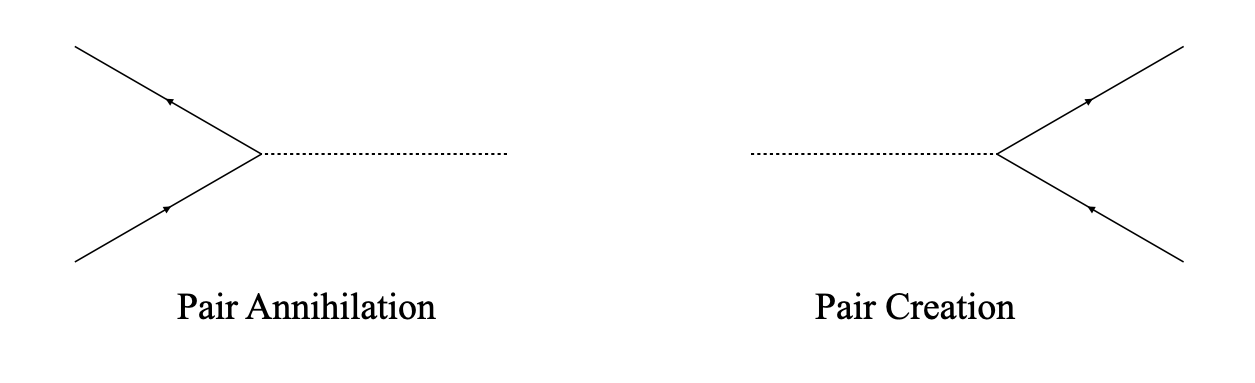
\includegraphics[width = 0.7\linewidth]{figures/creation_annihilate.png}
    \caption{Feynman diagrams corresponding to equation \ref{H_pair}}
\end{figure}


In quantum field theory, particles can be spontaneously created or annihilated and modeling this behavior is relevant for \ws{insert why this is useful here @gus}.
\textit{Feynman diagrams} are often used in high-energy physics to describe such these events.
In Figure \ref{fig:feynman}, a Feynman diagram is used to show a particle-antiparticle pair annihilating one another to produce a new particle (left) or how another particle can decay and produce a particle-antiparticle pair (right).

An example Hamiltonian that can be used to model a series of interactions of this form is given by:
\begin{equation}
    \label{eq:pairing-hamiltonian}
    H = \sum_n^{I} b_n^\dagger b_n + \sum_n^{I} d_n^\dagger d_n + \sum_n^{I} a_n^\dagger a_n + g\sum_{i,j,k}^{I} \left(b_i^\dagger d_j^\dagger a_k + b_i d_j a_k^\dagger \right).
\end{equation}

The first three terms give the kinetic energies of the individual fermions, antifermions, and bosons respectively.
The last two term describe a pair creation event and a pair annihilation event respectively.
In the pair creation event, a fermion and antifermion pair is spontaneously created by the annihilation of a boson.
In the pair annihilation event, a fermion and antifermion pair is spontaneously annihilated, resulting in a boson being created. 
The variable $g$ is a scalar coupling constant that describes the strength of coupling between the fermions and bosons. 
There are two parameters that control the size of the system: the number of momentum modes ($I$) and the bosonic occupancy cutoff ($\Omega$).

\begin{figure}
    \centering
    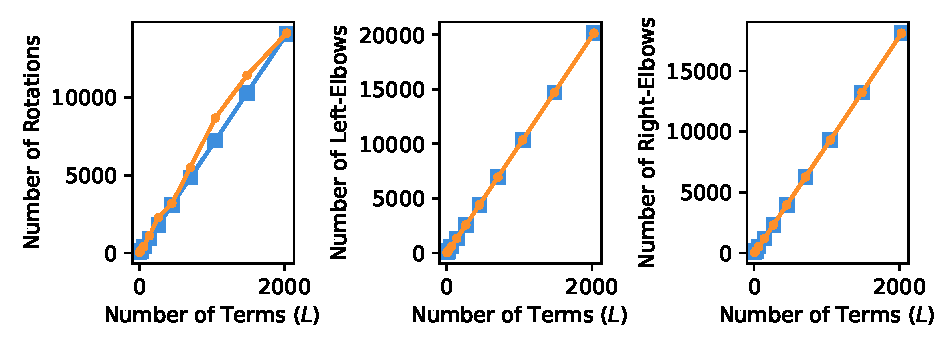
\includegraphics[width=16cm]{figures/pairing_hamiltonian_gates_vs_terms.pdf}
    \caption{
        \textbf{Numerical Gate Counts for Increasing $I$ (Pairing Hamiltonian).}
        The number of rotations (left), left-elbows (middle), and right-elbows (right) are plotted as a function of the number of terms in the Hamiltonian ($L$) for an increasing number of momentum modes ($I$).
        The gate counts for the variant of LOBE using \textit{USP} are shown as the blue squares.
        The gate counts for the variant of LOBE using \textit{ASP} are shown as the orange circles.
        The bosonic occupancy cutoff ($\Omega$) is set to $3$.
        The number of rotations excludes rotations by angles that result in Clifford operations.
    }
    \label{fig:pairing_hamiltonian_gates_vs_terms}
\end{figure}
\begin{figure}
    \centering
    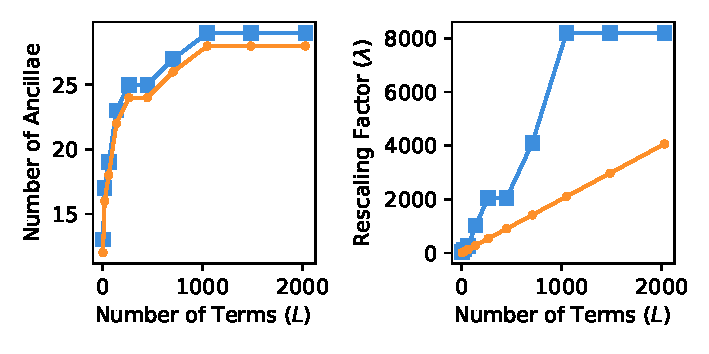
\includegraphics[width=12cm]{figures/pairing_hamiltonian_qubits_and_rescaling_vs_terms.pdf}
    \caption{
        \textbf{Numerical Ancillae Counts and Rescaling Factors for Increasing $I$ (Pairing Hamiltonian).}
        The number of required ancillae (left) and the resulting rescaling factor (right) for LOBE are plotted as a function of the number of terms in the Hamiltonian ($L$) for an increasing number of momentum modes ($I$).
        The counts for the variant of LOBE using \textit{USP} are shown as the blue squares.
        The counts for the variant of LOBE using \textit{ASP} are shown as the orange circles.
        The bosonic occupancy cutoff ($\Omega$) is set to $3$.
    }
    \label{fig:pairing_hamiltonian_qubits_and_rescaling_vs_terms}
\end{figure}

In Figure \ref{fig:pairing_hamiltonian_gates_vs_terms}, we plot the numerical gate counts estimates for the Pairing Hamiltonian (Eq. \ref{eq:pairing-hamiltonian}) as the number of terms in the Hamiltonain ($L$) increases.
The number of terms ($L$) increases directly with an increasing number of momentum modes and is given by $L = I^3 + 3I$ \ws{confirm this, im just eyeballing rn}.
For the three non-Clifford operations, the number of operations increases linearly with the number of terms in the Hamiltonian for this model.
Additionally, the two different compilation strategies (\textit{USP} (blue), \textit{ASP} orange) demonstrate the same numerical scaling and have nearly identical gate counts for all types of operations.
When the number of terms ($L$) is far from the next largest power of 2, \textit{ASP} requires more arbitrary rotations due to the compilation of Grover-Rudolph that is used in this work.

In Figure \ref{fig:pairing_hamiltonian_qubits_and_rescaling_vs_terms}, we plot the numerical estimates for the number of required ancillae (left) and the imposed rescaling factor (right) as the number of terms in the Hamiltonain ($L$) increases.
The number of ancillae grows logarithmically with the number of terms for both implementations.
The number of ancillae used for the index register grows logarithmically with the number of terms which accounts for this scaling.
The main advantage of the \textit{ASP} variant is the effect on the rescaling factor of the block-encoding.
While the rescaling factor of both variants seemingly grows linearly with respect to the number of terms in the Hamiltonian, the rescaling factor for the \textit{ASP} variant is significantly smaller than the \textit{USP} variant.
When block-encodings are employed as a subroutine in larger algorithms, the quantum resources for the algorithm are often dependent on the rescaling factor (with a lower rescaling factor generally being preferred).
For example, in the context of using Quantum Phase Estimation to estimate the eigenvalues of a Hamiltonian, the number of gates required typically scales as $O(\frac{1}{\lambda})$ \cite{babbush2018encoding}. 
However, the exact cost associated with the rescaling factor is difficult to determine without choosing a specific algorithm to benchmark with.

\begin{figure}
    \centering
    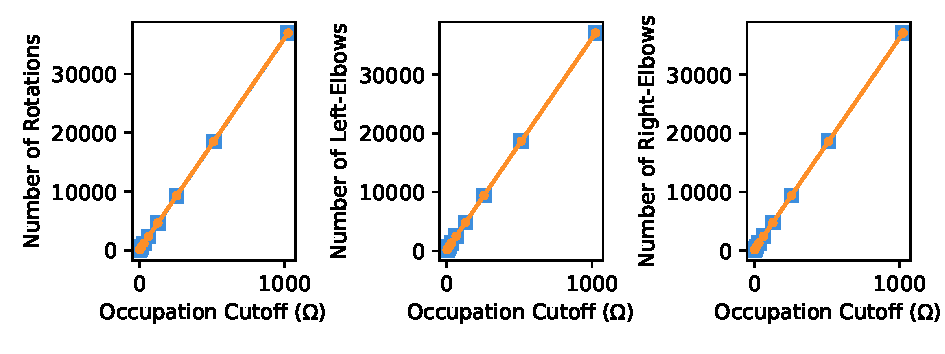
\includegraphics[width=16cm]{figures/pairing_hamiltonian_gates_vs_omega.pdf}
    \caption{
        \textbf{Numerical Gate Counts for Increasing $\Omega$ (Pairing Hamiltonian) .}
        The number of rotations (left), left-elbows (middle), and right-elbows (right) are plotted as a function of the bosonic occupation cutoff ($\Omega$).
        The gate counts for the variant of LOBE using \textit{USP} are shown as the blue squares.
        The gate counts for the variant of LOBE using \textit{ASP} are shown as the orange circles.
        The number of momentum modes ($I$) is set to $2$.
        The number of rotations excludes rotations by angles that result in Clifford operations.
    }
    \label{fig:pairing_hamiltonian_gates_vs_omega}
\end{figure}
\begin{figure}
    \centering
    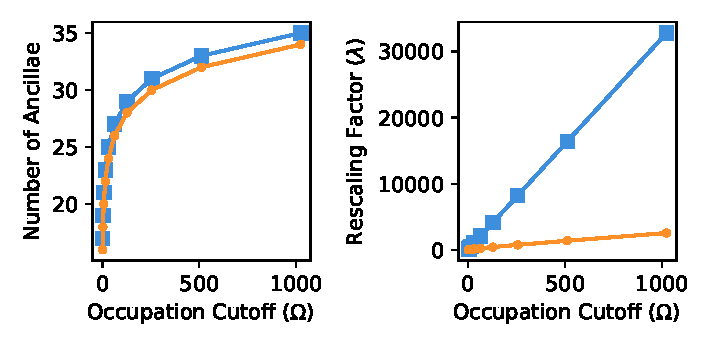
\includegraphics[width=12cm]{figures/pairing_hamiltonian_qubits_and_rescaling_vs_omega.pdf}
    \caption{
        \textbf{Numerical Ancillae Counts and Rescaling Factors for Increasing $\Omega$ (Pairing Hamiltonian).}
        The number of required ancillae (left) and the resulting rescaling factor (right) for LOBE are plotted as a function of the bosonic occupation cutoff ($\Omega$).
        The counts for the variant of LOBE using \textit{USP} are shown as the blue squares.
        The counts for the variant of LOBE using \textit{ASP} are shown as the orange circles.
        The number of momentum modes ($I$) is set to $2$.
    }
    \label{fig:pairing_hamiltonian_qubits_and_rescaling_vs_omega}
\end{figure}

In Figure \ref{fig:pairing_hamiltonian_gates_vs_omega}, we plot the numerical gate counts estimates for the Pairing Hamiltonian (Eq. \ref{eq:pairing-hamiltonian}) as the cutoff on the maximum bosonic occupation ($\Omega$) increases.
For the three non-Clifford operations, the number of operations increases linearly with the bosonic occupancy cutoff for this model.
Similar to the case with increasing $I$, the two different compilation strategies (\textit{USP} (blue), \textit{ASP} orange) demonstrate the same numerical scaling and have nearly identical gate counts for all types of operations.

In Figure \ref{fig:pairing_hamiltonian_qubits_and_rescaling_vs_omega}, we plot the numerical estimates for the number of required ancillae (left) and the imposed rescaling factor (right) as the cutoff on the maximum bosonic occupation ($\Omega$) increases.
The number of ancillae grows logarithmically with the bosonic occupation cutoff for both implementations.
The number of ancillae needed to update the bosonic occupancy grows logarithmically with $\Omega$ (Eq. \ref{eq:ancillae-bosonic-updates}) which accounts for this scaling.
Again, the main advantage of the \textit{ASP} variant is that the imposed rescaling factor is significantly smaller than the \textit{USP} variant, especially for large values of $\Omega$ despite the asymptotic scaling being linear for both.
